\documentclass[conference]{IEEEtran}

\usepackage{cite}
\usepackage{amsmath}
\usepackage{graphicx}
\usepackage{url}
\usepackage[hidelinks]{hyperref}

\begin{document}

\title{Beyond Compilation: Functional Correctness and Static-Analysis Compliance in LLM-Generated TypeScript}

\author{\IEEEauthorblockN{Yehezkiel Gunawan}
\IEEEauthorblockA{Bina Nusantara University\\
Jakarta, Indonesia\\
yehezkiel.gunawan@binus.ac.id}}

\maketitle

\begin{abstract}
An LLM-generated TypeScript program may fail strict compilation, compile but violate a behavioral requirement, or pass its tests while violating selected project-level static-analysis rules. We examined these outcomes separately using 15 deterministic TypeScript utility tasks, three models, and 45 generated programs. Each program underwent source extraction, safety inspection, and strict TypeScript compilation; compilable programs then proceeded to task-specific Vitest tests and ESLint analysis. Of the 45 programs, 37 compiled, 36 passed all visible tests, and 34 passed the complete evaluation gate. All eight compilation failures involved possibly undefined indexed access under strict TypeScript settings. Testing rejected one additional compilable program, and ESLint identified violations in two programs that had passed every visible test. In the evaluated tasks and models, compilation, functional correctness, and compliance with selected static-analysis rules were distinct outcomes. Compilation was a useful first filter, but it did not replace behavioral testing or project-specific static analysis.
\end{abstract}

\begin{IEEEkeywords}
large language models, code generation, TypeScript, functional correctness, static analysis, empirical software engineering
\end{IEEEkeywords}

\section{Introduction}
A TypeScript program generated by a large language model (LLM) may fail strict compilation, compile but violate a behavioral requirement, or pass its tests while violating project-level static-analysis rules. These outcomes form three sequential but non-equivalent gates: compilation, functional tests, and selected static analysis. TypeScript makes the first distinction especially visible. Code that appears executable as JavaScript can still fail a strict type contract when indexed values, optional properties, or generic types retain the possibility of \texttt{undefined}.

Execution-based benchmarks such as HumanEval made tests central to code-generation evaluation \cite{chen2021humaneval}. Later studies examined variation across languages and models, properties beyond functional correctness, and tasks extending from function synthesis to repository issue resolution \cite{xu2022systematic,nguyen2022copilot,yetistiren2022quality,du2024classeval,jimenez2024swebench}. Comparatively less attention has been given to compact, reproducible evaluations of strict TypeScript utilities that report compilation, behavioral, and static-analysis outcomes separately. This study addresses that narrower gap as an incremental empirical contribution.

The benchmark uses 15 deterministic utilities that are independently testable and small enough for source-level inspection. They represent common TypeScript development concerns while excluding frameworks, databases, browsers, and external services that would add competing explanations for failure.

This study asks how reliably contemporary LLMs produce TypeScript that survives three conventional development checks. We address the following questions:

\textit{RQ1: To what extent does generated TypeScript compile under strict compiler settings?}

\textit{RQ2: To what extent are compilable programs functionally correct under task-specific tests?}

\textit{RQ3: What violations of selected static-analysis rules remain, including in programs that pass all tests?}

The contribution is a reproducible TypeScript corpus, a controlled 45-generation comparison under one prompt, and an empirical account of attrition across the three gates. The artifact, including tasks, prompts, raw generations, evaluation records, and report scripts, is available online.\footnote{\url{https://github.com/yehezkielgunawan/icdees-2026}}

\section{Related Work}
\subsection{Functional correctness}
HumanEval established execution against unit tests as a standard measure for function synthesis \cite{chen2021humaneval}. Xu et al. found substantial variation across code models and programming languages \cite{xu2022systematic}, while Nguyen and Nadi evaluated Copilot suggestions with tests and complexity measures \cite{nguyen2022copilot}. The test oracle determines how much this evidence establishes: EvalPlus exposed programs accepted by the original HumanEval tests after expanding the suites \cite{liu2023evalplus}. Our tests therefore measure conformance to specified cases rather than proof of correctness.

\subsection{Properties beyond functional correctness}
Passing tests does not establish every relevant property of generated code. Yeti\c{s}tiren et al. assessed several quality dimensions \cite{yetistiren2022quality}, Al Madi examined readability and complexity \cite{almadi2022readable}, and Pearce et al. evaluated security \cite{pearce2022security}. Our ESLint stage has a narrower construct: compliance with selected project rules, not maintainability, security, or production readiness.

\subsection{Robustness and nondeterminism}
Generation conditions affect reproducibility. Semantically similar prompts can change Copilot outputs \cite{mastropaolo2023robustness}; prompt language and repeated runs can alter suggestion outcomes \cite{koyanagi2024languages}. Ouyang et al. report nondeterminism in ChatGPT code generation \cite{ouyang2025nondeterminism}. We therefore fixed one prompt and retained the generated artifacts. This control removes prompt strategy as an independent variable, but one generation per model-task pair cannot characterize output variability.

\subsection{Software-engineering task scope}
Evaluation now spans isolated functions, class-level generation, repository issue resolution, and agents that edit repositories and run development commands \cite{chen2021humaneval,du2024classeval,jimenez2024swebench,yang2024sweagent}. Our smaller utilities trade application-level realism for deterministic execution, manual inspectability, and isolation of strict TypeScript behavior. They provide ecosystem-specific evidence rather than another general-purpose benchmark, consistent with the range of evaluation practices catalogued by Hou et al. \cite{hou2024slr}.

\section{Method}
\subsection{Research design and tasks}
The independent variable was the model. Dependent variables were strict compilation, full test-suite success, selected ESLint findings, and passage through all gates. The task, prompt, execution order, test suite, compiler, lint rules, and dependency lock were held constant across models.

The corpus contains 15 tasks divided evenly among five categories (Table~\ref{tab:tasks}). Selection required deterministic behavior, independent testability, bounded source size, manual inspectability, and relevance to TypeScript or web-backend development. Examples include building a category tree, validating pagination parameters, normalizing URL paths, limiting asynchronous concurrency, and implementing cursor pagination. We excluded React, Next.js, databases, browsers, and external APIs so that framework behavior, environment state, and remote services would not confound the three measured outcomes. Each task has a required exported signature, a reference implementation, and four to six Vitest cases. The corpus contains 75 tests in total. Reference implementations passed all tests, strict compilation, and ESLint under the same evaluator.

\begin{table}[!h]
\caption{TypeScript task set}
\label{tab:tasks}
\centering
\scriptsize
\begin{tabular}{@{}p{0.30\columnwidth}cp{0.49\columnwidth}@{}}
\hline
\textbf{Category} & \textbf{No.} & \textbf{Representative task} \\
\hline
Data transformation & 3 & Group records by a derived key \\
Validation & 3 & Validate a registration form \\
String and URL processing & 3 & Convert a title to a URL-safe slug \\
Async and Promise utilities & 3 & Retry an asynchronous operation \\
Web backend utilities & 3 & Implement an in-memory TTL cache \\
\hline
\end{tabular}
\end{table}


\subsection{Generation procedure}
We evaluated three identifiers from the OpenAI provider: \texttt{gpt-5.6-sol}, \texttt{gpt-5.6-terra}, and \texttt{gpt-5.6-luna}, labeled Sol, Terra, and Luna. These identifiers were active in the recorded provider snapshot but do not identify immutable public model revisions. Each model generated one program for each task, for 45 generations. The campaign ran on September 3, 2026 through OpenCode 1.18.26.

One prompt template required source code only, the exact signature, no imports or external dependencies, no \texttt{any}, no TypeScript suppression comments, and no process, file-system, network, or global mutable-state access. Holding this template constant prevented prompt strategy from becoming another independent variable. The benchmark agent could not call tools and was limited to one step. A temperature of zero was requested, but the runtime marked temperature unsupported for all three models and recorded no applied value. The configured 4096-token output limit was recorded but not transmitted by the generation call, so it is not treated as an enforced control. The campaign manifest froze the task inputs, prompt, study configuration, and dependency lockfile before generation, preventing post-hoc changes to those inputs. All raw responses, extracted sources, hashes, and metadata were retained. All 45 generations and extractions succeeded without normalization changes.

\subsection{Evaluation pipeline}
The evaluator first checked for empty output and disallowed operations. It then compiled each candidate and its tests with TypeScript 5.8.2 using \texttt{strict}, \texttt{noImplicitAny}, \texttt{noUncheckedIndexedAccess}, and \texttt{exactOptionalPropertyTypes}, among other module-isolation settings. Strict compilation tests whether generated TypeScript satisfies a stronger static contract than successful JavaScript execution. Compile failure stopped later stages. Compilable candidates proceeded to their Vitest 3.2.4 suite and ESLint 9.35.0 in parallel. Deterministic visible tests provided reproducible checks of specified behavior, while ESLint supplied a lightweight, reproducible check of selected project rules.

A candidate was \emph{fully correct} when at least one test ran and every test passed. A candidate was \emph{static-clean} when ESLint completed with zero errors. Selected rules included a cyclomatic-complexity maximum of 12, \texttt{prefer-const}, equality and control-flow rules, and TypeScript rules for explicit \texttt{any} and unused variables. The \emph{full gate} required successful extraction, compilation, full correctness, and zero ESLint errors. Compilation, functional, and full-gate rates use all generations as their denominator. Static-clean and compiled-but-incorrect rates use compilable programs; correct-but-static-issue rates use fully correct programs. Given 15 paired tasks and one sample per cell, we report counts and percentages without hypothesis tests or model-ranking claims.

\section{Results}
Table~\ref{tab:results} reports each model and the aggregate outcomes. Fig.~\ref{fig:gates} shows the same sequential gates to make attrition explicit.

\begin{table*}[t]
\caption{Results by model. Compilation, full correctness, and full gate use generated candidates as denominators. Static-clean and compiled-incorrect use compiled candidates; correct-static-issue uses fully correct candidates.}
\label{tab:results}
\centering
\small
\begin{tabular}{lcccccc}
\hline
\textbf{Model} & \textbf{Compiled} & \textbf{Fully correct} & \textbf{Static-clean} & \textbf{Full gate} & \textbf{Compiled, incorrect} & \textbf{Correct, static issue} \\
\hline
GPT-5.6 Sol & 12/15 (80.0\%) & 12/15 (80.0\%) & 12/12 (100.0\%) & 12/15 (80.0\%) & 0/12 (0.0\%) & 0/12 (0.0\%) \\
GPT-5.6 Terra & 12/15 (80.0\%) & 11/15 (73.3\%) & 11/12 (91.7\%) & 10/15 (66.7\%) & 1/12 (8.3\%) & 1/11 (9.1\%) \\
GPT-5.6 Luna & 13/15 (86.7\%) & 13/15 (86.7\%) & 12/13 (92.3\%) & 12/15 (80.0\%) & 0/13 (0.0\%) & 1/13 (7.7\%) \\
\hline
\textbf{All} & \textbf{37/45 (82.2\%)} & \textbf{36/45 (80.0\%)} & \textbf{35/37 (94.6\%)} & \textbf{34/45 (75.6\%)} & \textbf{1/37 (2.7\%)} & \textbf{2/36 (5.6\%)} \\
\hline
\end{tabular}
\end{table*}


\begin{figure*}[t]
\centering
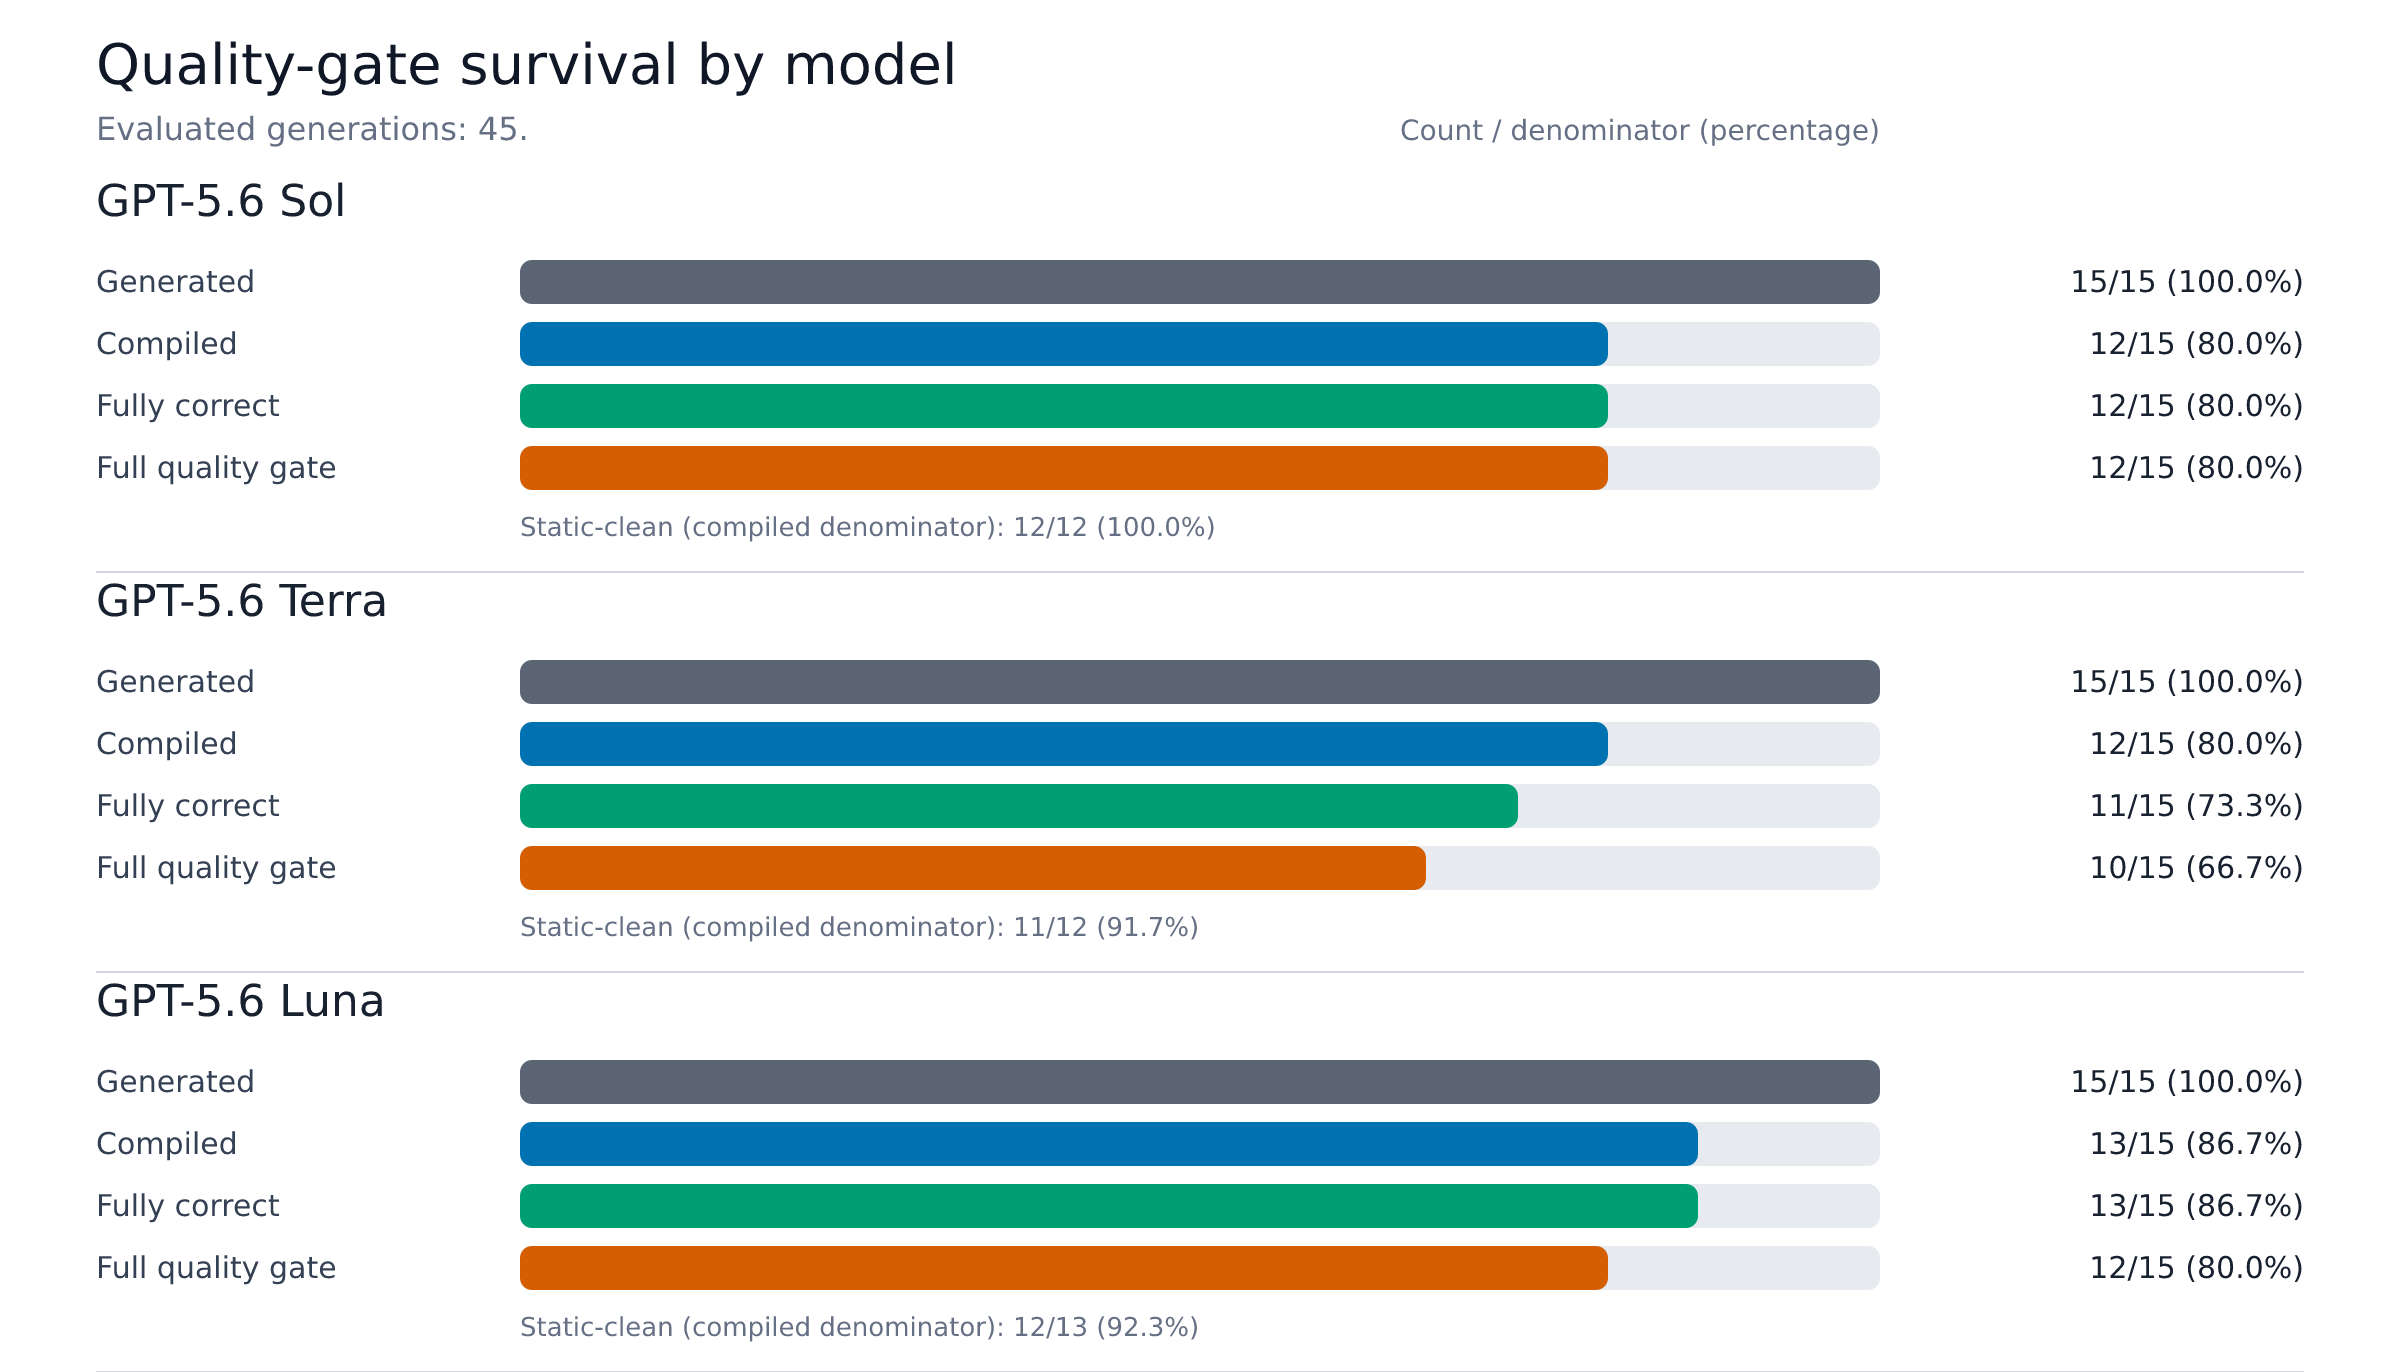
\includegraphics[width=0.92\textwidth]{figures/figure-1-quality-gates.png}
\caption{Quality-gate survival for the 45 primary generations. Static-clean rates are shown separately because their denominator is the number of compilable candidates.}
\label{fig:gates}
\end{figure*}

\subsection{RQ1: Strict compilation}
Thirty-seven of 45 candidates compiled, an aggregate rate of 82.2\%. The observed model rates ranged from 12/15 (80.0\%) for Sol and Terra to 13/15 (86.7\%) for Luna. Every rejected candidate had exactly one compiler error, and all eight errors involved possibly undefined indexed access under \texttt{noUncheckedIndexedAccess}.

The failures were concentrated in three tasks rather than spread across the corpus. Sol and Terra failed task 08 by constructing an array whose inferred element type remained \texttt{string | undefined}. All three models failed task 11 when passing \texttt{items[index]}, typed as \texttt{T | undefined}, to a worker expecting \texttt{T}. All three failed task 15 through a similar access to the last page item. These are strict type failures, not observed test failures: the pipeline did not run Vitest or ESLint after compilation failed.

\subsection{RQ2: Functional correctness}
Among 37 compilable candidates, 36 passed their complete task suite (97.3\%). Relative to all generated candidates, the functional success rate was 36/45 (80.0\%). Across compiled programs, 178 of 179 executed test cases passed, but candidate-level outcomes remain the unit of analysis.

The sole compiled-but-incorrect candidate was Terra's registration validator in task 04. It passed four of five tests. For an empty object, it reported missing username, email, and password fields but omitted \texttt{confirmPassword}. Both password fields evaluated to \texttt{undefined}, so their strict equality comparison returned \texttt{true}. This case directly separates compilation from behavioral compliance, although its frequency, 1/37, does not support a claim that compiled programs often failed the tests.

\subsection{RQ3: Static-analysis compliance and the full gate}
Thirty-five of 37 compiled candidates were static-clean (94.6\%). Both lint failures had passed all functional tests. Luna's URL-path normalizer had cyclomatic complexity 13 against the configured maximum of 12. Terra's Promise-timeout utility declared a reassignment-free timer with \texttt{let}, violating \texttt{prefer-const}. No linted candidate used explicit \texttt{any}, suppression comments, or generated a warning.

The static stage reduced the fully correct set from 36 to 34 full-gate programs. Sol and Luna each passed the complete gate for 12/15 candidates (80.0\%); Terra passed for 10/15 (66.7\%). These differences are descriptive observations from one run, not estimates of stable model ordering.

\section{Discussion}
\subsection{Compilation is useful but incomplete}
Compilation rejected eight programs before behavioral evaluation. Every failure reflected the same TypeScript-specific problem: runtime reasoning about bounds or existence did not narrow an indexed value enough to satisfy its declared type. Values remained \texttt{T | undefined} or \texttt{string | undefined} until the implementation supplied explicit narrowing or a justified non-null assertion. The generated logic could appear executable while failing TypeScript's static proof requirements.

In this corpus, strict compilation eliminated more candidates than the subsequent visible test suites, which rejected one additional compilable program. This comparison identifies compilation as an effective first filter for these tasks, not as a generally stronger validation method. The registration defect shows why the distinction matters: a program can satisfy the type checker and still violate a boundary-case requirement.

\subsection{Behavioral tests and static analysis answer different questions}
Terra's validator treated two missing password fields as equal because both evaluated to \texttt{undefined}. The program was type-correct, but a visible test exposed the omitted validation error. Test evidence remains finite: EvalPlus has shown that expanded suites can reject programs accepted by smaller suites \cite{liu2023evalplus}. Here, ``fully correct'' means success on four to six visible tests, not proof against the complete input space.

The two ESLint findings occurred in test-passing programs and did not indicate behavioral defects. One captured a reassignment-free \texttt{let}; the other marked complexity one point above the configured threshold. They show that test success does not imply compliance with selected project rules. They do not establish maintainability, security, or production readiness, which require broader measures and, in some cases, human assessment.

\subsection{Conventional engineering gates remain useful}
Generated TypeScript should be treated as candidate code and subjected to the same compiler, tests, and static-analysis checks as human-written code. Each gate answers a different question: strict compilation checks the type contract, tests exercise specified behavior, and ESLint enforces selected project rules. Explicit denominators are also necessary because compile failures never reach later stages. Reporting a static-clean rate over all generations would conflate rejection with unobserved lint behavior.

\section{Scope, Limitations, and Threats to Validity}
This study covers 45 single-attempt generations across 15 isolated TypeScript utility tasks and three provider model identifiers. It measures strict compilation, performance on visible task-specific tests, and compliance with selected ESLint rules. The findings characterize this controlled campaign; they do not establish general LLM coding performance, production readiness, or stable differences among models.

\textit{Construct validity.} Unit tests approximate functional correctness and cover only four to six cases per task. One task description included URL query and fragment handling that its tests did not exercise, which further limits the ``fully correct'' label. ESLint represents a small set of static rules, not general maintainability or security. Strict compilation failures mainly measure explicit handling of conservative indexed-access types and should not be interpreted as algorithmic errors.

\textit{Internal and conclusion validity.} Each model-task pair has one generation. Because temperature control was unsupported, the study cannot separate stable model behavior from sampling variation. Fixed prompts and complete raw-output capture improve auditability but do not remove nondeterminism or provider updates \cite{mastropaolo2023robustness,ouyang2025nondeterminism}. The small paired sample precludes strong ranking claims. The manifest froze tasks, prompt, study configuration, and a dependency lockfile, but did not bind the evaluator source revision or benchmark-agent configuration. The exact campaign-time Node version, operating system, and provider-side model revisions were not captured.

\textit{External validity.} The corpus contains 15 isolated TypeScript utilities, three provider identifiers, one prompt, and visible tests. Results do not generalize to full applications, interactive assistants, repository agents, other languages, or other model revisions. The compact design improves control and reproducibility but is less realistic than class-level or repository-level benchmarks.

\section{Conclusion}
Among 45 generated TypeScript programs, strict compilation rejected eight, testing exposed one additional behavioral defect, and ESLint identified selected rule violations in two otherwise test-passing programs. These outcomes show that compilation, functional correctness, and static-analysis compliance were distinct gates for the evaluated tasks and models. Compilation was an effective first filter in this corpus, but neither compilation nor test success established passage through the complete evaluation pipeline. Generated TypeScript should therefore undergo ordinary project validation before integration.

\section*{Acknowledgment}
The author used OpenCode with GPT-5.6-sol and GPT-5.6-luna primarily for technical coding tasks; support for the systematic literature review through Exa AI MCP, including source discovery, metadata verification, and source organization; and language editing, including paraphrasing and correction of language errors. The author independently reviewed and validated all AI-assisted outputs, verified the empirical claims and cited sources, and assumes full responsibility for the accuracy, interpretation, and final content of the manuscript.


\IEEEtriggeratref{7}
\bibliographystyle{IEEEtran}
\bibliography{references}

\end{document}
